\section{Results}\label{sect:results}

\begin{itemize}
    \item Images of select cases, demonstrating segmentation process
\end{itemize}

The computed volumes of the prostates from the MR and ARFI imaging data are
presented in Table~\ref{tab:mr_arfi_volumes}.  The subvolumes associated
with the zonal anatomy in each imaging modality was measured
(Figure~\ref{fig:mr_arfi_volumes}(a)), showing an mean overestimation of
total prostate volume of 36.7 $\pm$ 27.9\% by ARFI imaging compared to MR
volumes (Figure~\ref{fig:mr_arfi_volumes}(b)), and a relative
underestimation of the central zone volume relative to the central gland in MR
imaging of -15.3 $\pm$ 13.0 \% (Figure~\ref{fig:mr_arfi_volumes}(c)).

\begin{table}
\centering
\caption{Comparison of Central Gland / Zone and Total Prostate Volumes in MR T2WI and ARFI Imaging}
\begin{tabular}{|l|l|l|l|l|} \hline
{\bf Study Subject} & {\bf MR Central Gland} & {\bf MR Total} & {\bf ARFI Central Zone} & {\bf ARFI Total} \\ 
& {\bf Volume (mm$^3$)} & {\bf Volume (mm$^3$)} & {\bf Volume (mm$^3$)} & {\bf Volume (mm$^3$)} \\ \hline
P86 & 12738.12 & 24567.06 & 14296. & 40031. \\
P79 & 14263.86 & 28514.79 & 8370 & 33978 \\
P78 & 23471.81 & 32484.36 & 13290.47 & 37420 \\
P77 & 17317.03 & 32492.83 & 10829.7 & 31819 \\
P75 & 57561.69 & 70950.98 & 30369 & 73684.64 \\
P74 & 12010.3 & 27841.21 & 15679 & 43298.34 \\
P72 & 8824.44 & 19587.02 & 11776.44 & 28545.79 \\
P71 & 10969.65 & 21276.98 & 16020.73 & 31424.61 \\
P70 & 13633.36 & 20749.91 & 19282 & 36876.3\\
P69 & 23580.12 & 36112.58 & 33500 & 70654 \\
P67 & 16569.17 & 27332.39 & 25219 & 34656.2 \\
P61 & 25381.36 & 49213.93 & 18137 & 54044.3 \\
P59 & 9247.34 & 26360.37 & 6144 & 35137 \\
P58 & 14787.88 & 23361.47 & 19654.6 & 35211 \\
P57 & 17872.15 & 35371.12 & 10153 & 38028.47 \\
P56 & 33315.41 & 48495.39 & 39351 & 66425 \\ \hline
\end{tabular}
\label{tab:mr_arfi_volumes}
\end{table}


\begin{figure}[htb!]
\centering
\begin{tabular}{ccc}
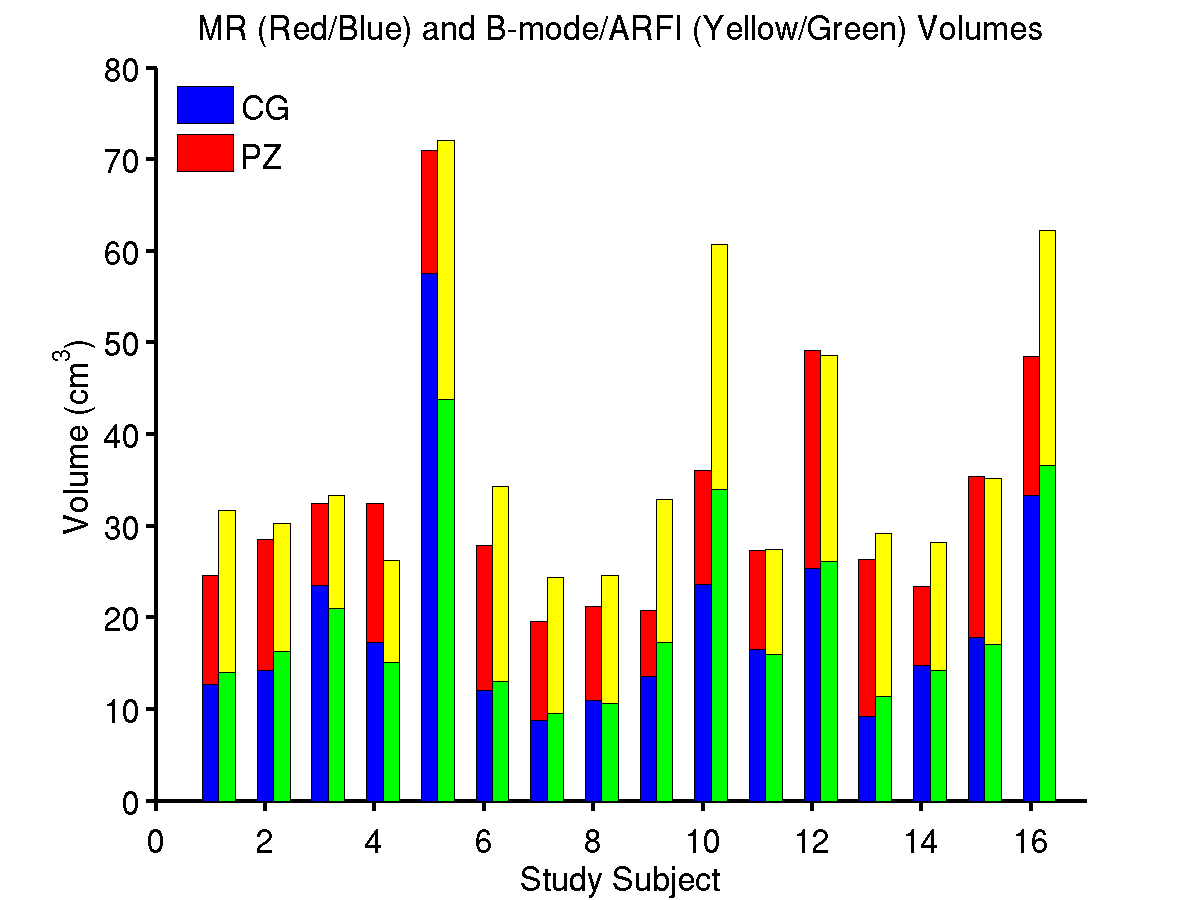
\includegraphics[width=0.3\linewidth]{figs/mr_arfi_volumes} &
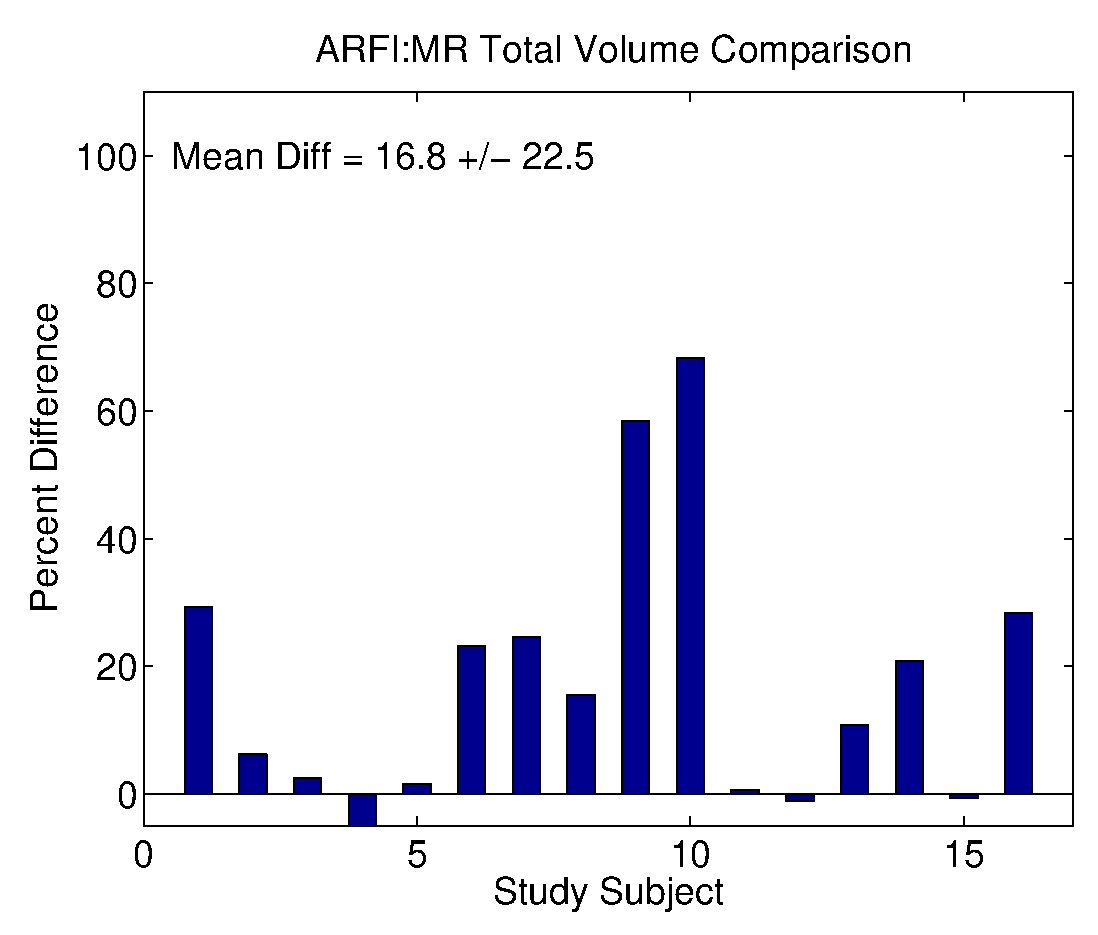
\includegraphics[width=0.3\linewidth]{figs/mr_arfi_volume_diff} &
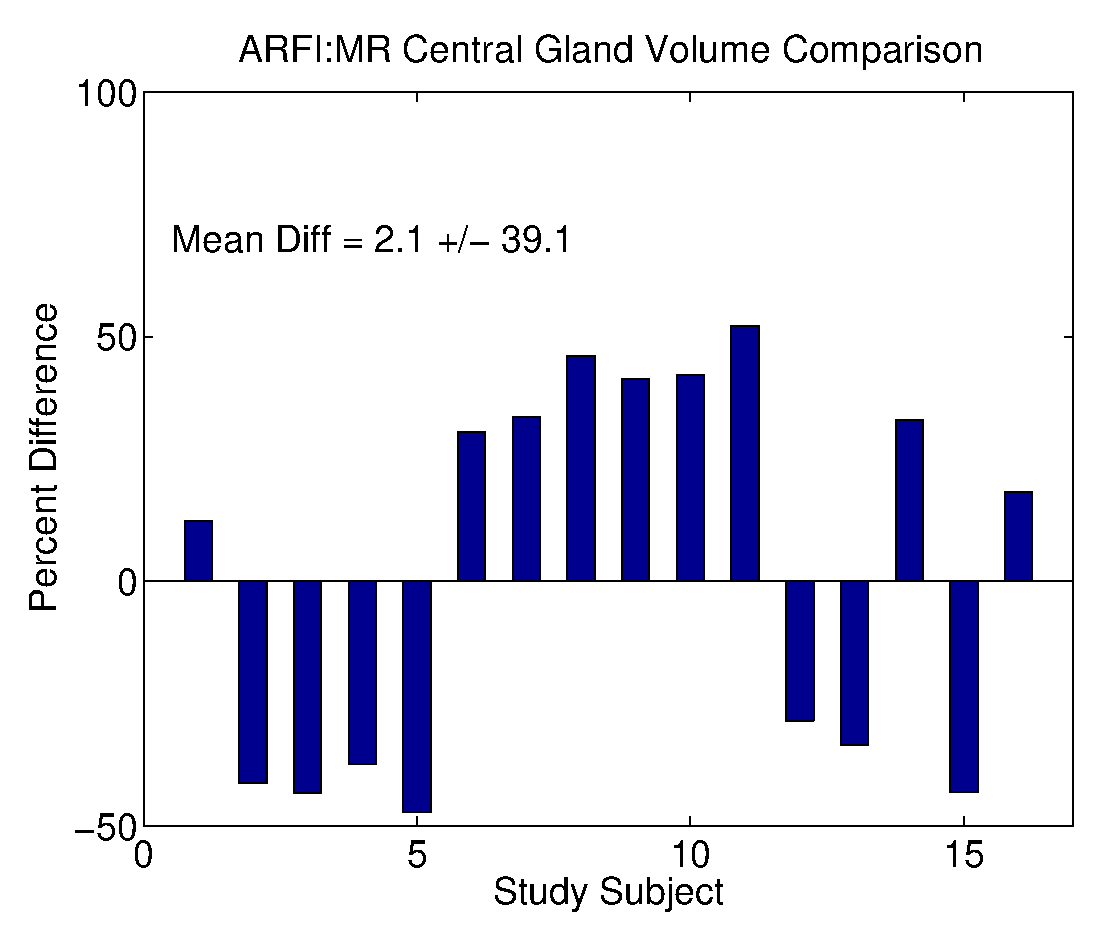
\includegraphics[width=0.3\linewidth]{figs/mr_arfi_central_diff} \\
(a) Central:Peripheral Volume & (b) Total Volume Difference & (c) Central Volume Difference\\
\end{tabular}
\caption{Comparison of MR and ARFI zonal anatomy volume estimates from
    manually-segmented images.  Total prostate volumes ranged from 19.6--71.0
    cm$^3$ based on MR image models (a), with ARFI image models overestimating
    total prostate volume by 36.7 $\pm$ 27.9\% (b).  ARFI image estimation of
    the central zone volume relative to the MR central gland volume varied by
    2.1 $\pm$ 39.0\% (c).  Table~\ref{tab:mr_arfi_volumes} contains the
    individual volume estimates for the entire prostate and the central
    glands.}
\label{fig:mr_arfi_volumes} 
\end{figure}


Weights and axis measurements from the gross pathology processing of the
excised prostates were collected (Table~\ref{tab:path_data}), and using the
axis measurements (lateral-to-lateral, anterior-to-posterior, and
apex-to-base), the prostate volume was approximated as a tri-axial ellipsoid,
and its volume was estimated.

\begin{table}[h!]
\centering
\caption{Pathology Prostate Gross Specimen Metrics}
\begin{tabular}{|l|l|l|l|l|l|} \hline
{\bf Study } & {\bf Weight} & {\bf Lat-Lat} & {\bf Anterior-} & {\bf Apex-Base} & {\bf Ellipsoidal} \\
{\bf Subject} & {\bf (g)} & {\bf (cm)} & {\bf Posterior (cm)} & {\bf (cm)} & {\bf Volume (cm$^3$)} \\ \hline
1 & 37. & 4.3 & 4.0 & 2.9 & 26.10 \\ 
2 & 52. & 4.5 & 3.5 & 3.5 & 28.85 \\ 
3 & 38. & 4.5 & 4.0 & 3.7 & 34.85 \\ 
4 & 84. & 7.0 & 6.5 & 6.0 & 142.87 \\ 
5 & 72. & 6.6 & 4.3 & 3.0 & 44.56 \\ 
6 & 49. & 4.9 & 4.4 & 3.4 & 38.36 \\ 
7 & 25. & 3.7 & 3.7 & 3.2 & 22.93 \\ 
8 & 27. & 4.2 & 3.1 & 2.7 & 18.40 \\ 
9 & 28. & 4.4 & 3.7 & 3.2 & 27.26 \\ 
10 & 42. & 4.7 & 3.5 & 3.2 & 27.55 \\ 
11 & 38. & 5.4 & 4.0 & 3.3 & 37.30 \\ 
12 & 50. & 5.0 & 4.0 & 3.7 & 38.73 \\ 
13 & 29. & 4.0 & 3.5 & 3.0 & 21.98 \\ 
14 & 27. & 4.5 & 3.0 & 3.0 & 21.20 \\ 
15 & 32. & 4.5 & 3.5 & 3.5 & 28.85 \\ 
16 & 62. & 5.5 & 5.3 & 5.2 & 79.33 \\ 

\hline
\end{tabular}
\label{tab:path_data}
\end{table}


MR and ARFI imaging total prostate volumes were also compared with the weights
and prostate volumes, approximated to be tri-axial ellipsoids, and calculated
from measurements of the prostate semi-principal axes.  Prostate weights were
moderately correlated with estimated pathology ellipsoidal prostate volumes
(Figure~\ref{fig:mr_arfi_weight}(a), R$^2$ = 0.68).  There was moderate
correlation between the prostate weight and the image-reconstructed prostate
volumes (Figure~\ref{fig:mr_arfi_weight}(b), R$^2$ = 0.44 (MR) and 0.21
(ARFI)), though there was weaker correlation with the ellipsoidal approximation
of the measurement prostate volume and the image-recontructed volumens
(Figure~\ref{fig:mr_arfi_weight}(c), R$^2$ = 0.08 (MR) and 0.01 (ARFI)).  

\begin{figure}[htb!]
\centering
\begin{tabular}{lll}
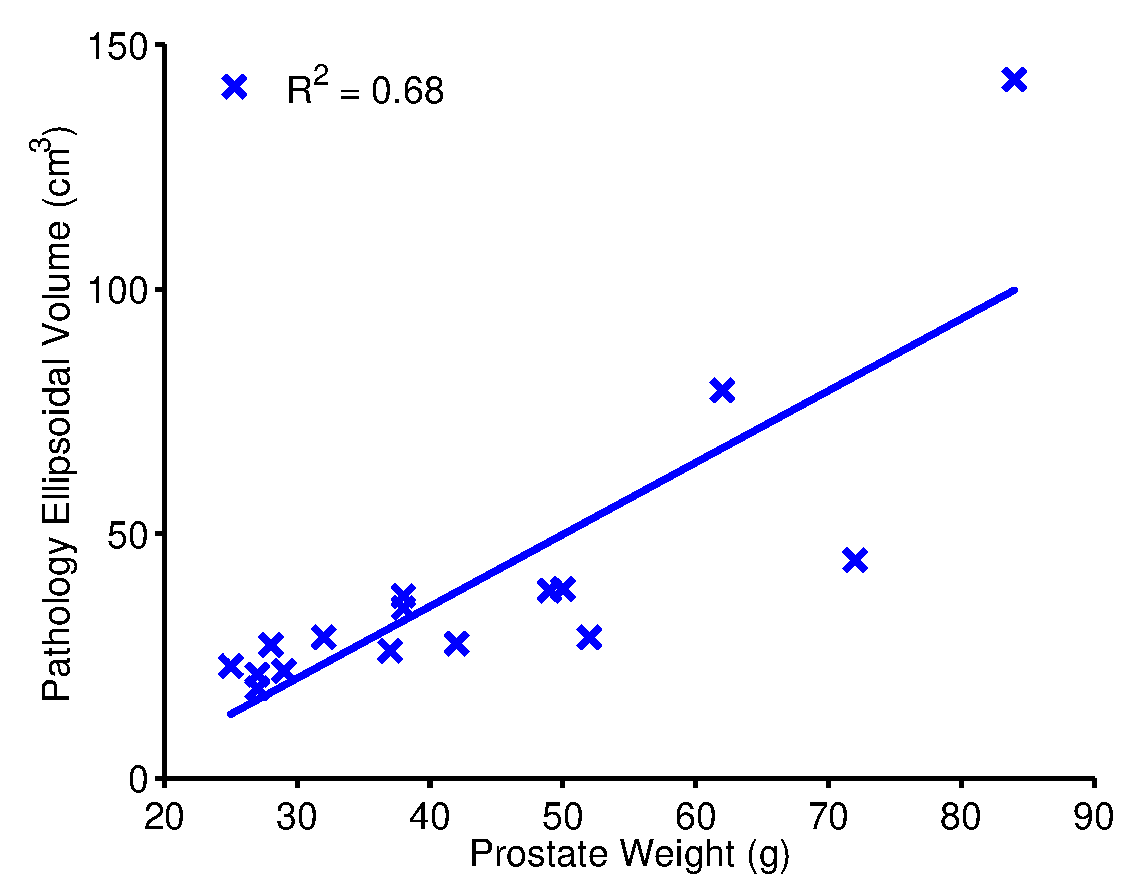
\includegraphics[width=0.3\linewidth]{figs/corr_path_vol_weight_vol} &
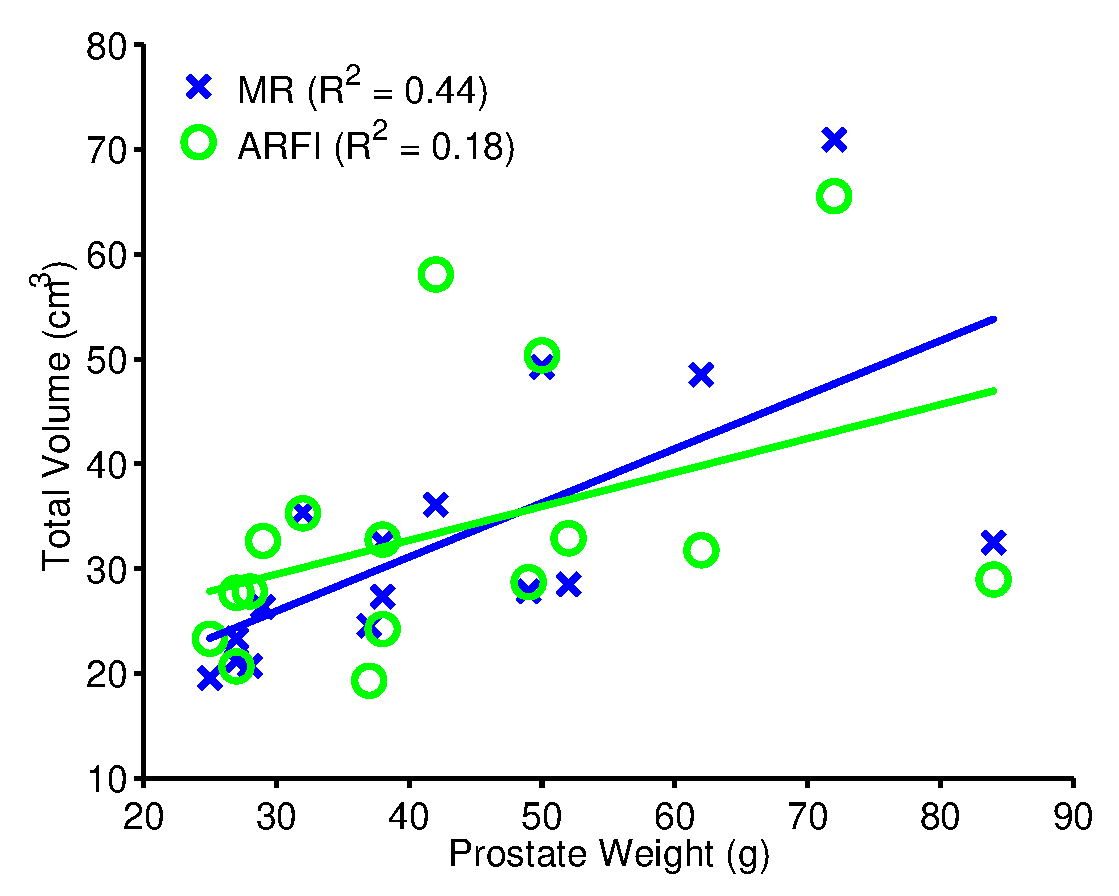
\includegraphics[width=0.3\linewidth]{figs/corr_weight_vol} &
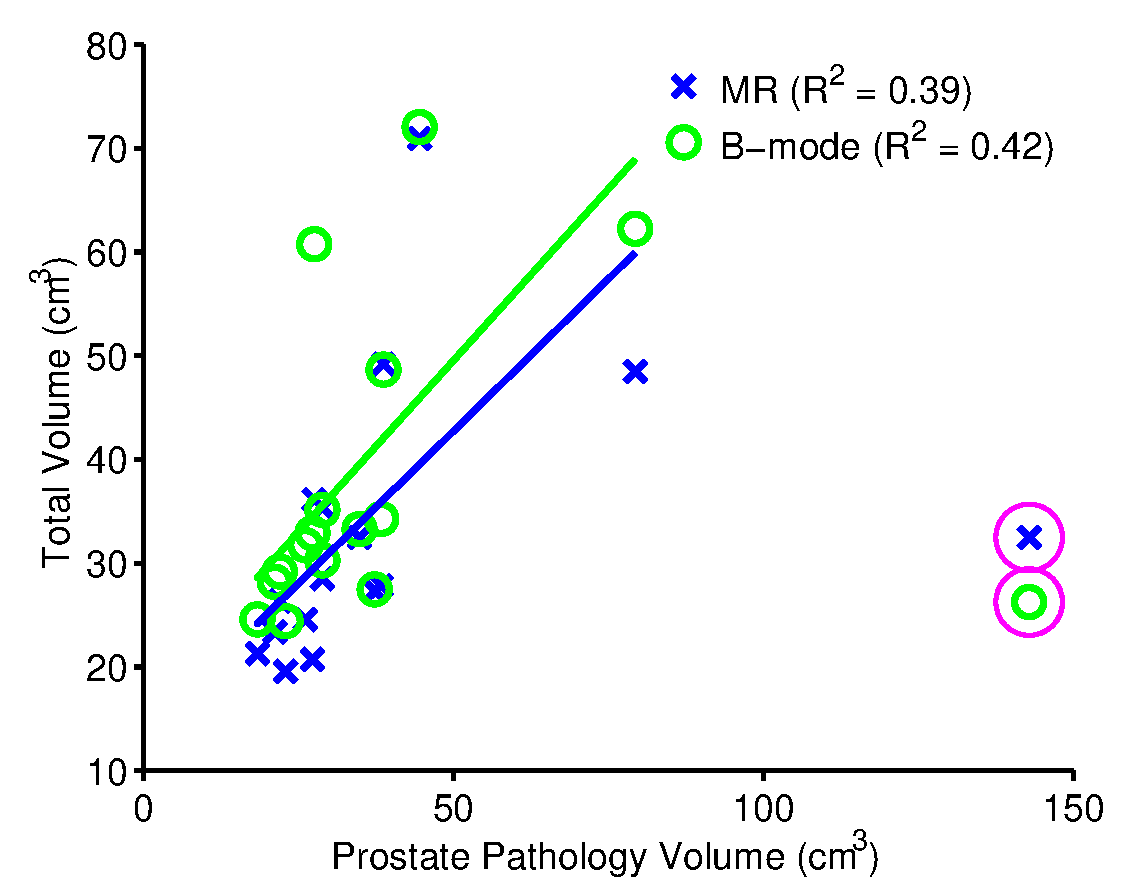
\includegraphics[width=0.3\linewidth]{figs/corr_pathVol_vol} \\
(a) Path Weight : Path Volume & (b) Image Volume : Prostate Weight & (c) Image Volume : Path Volume \\
\end{tabular}
%\begin{tabular}{ll}
%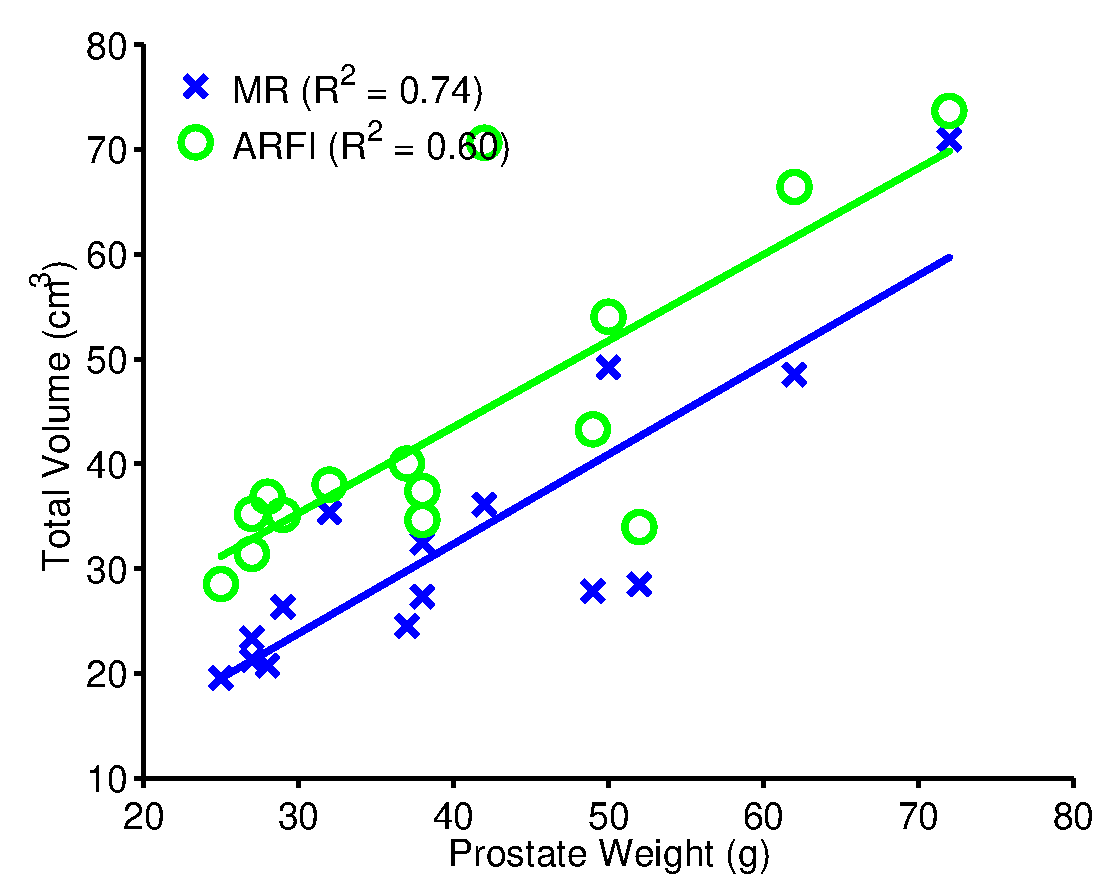
\includegraphics[width=0.3\linewidth]{figs/corr_weight_vol_no4} &
%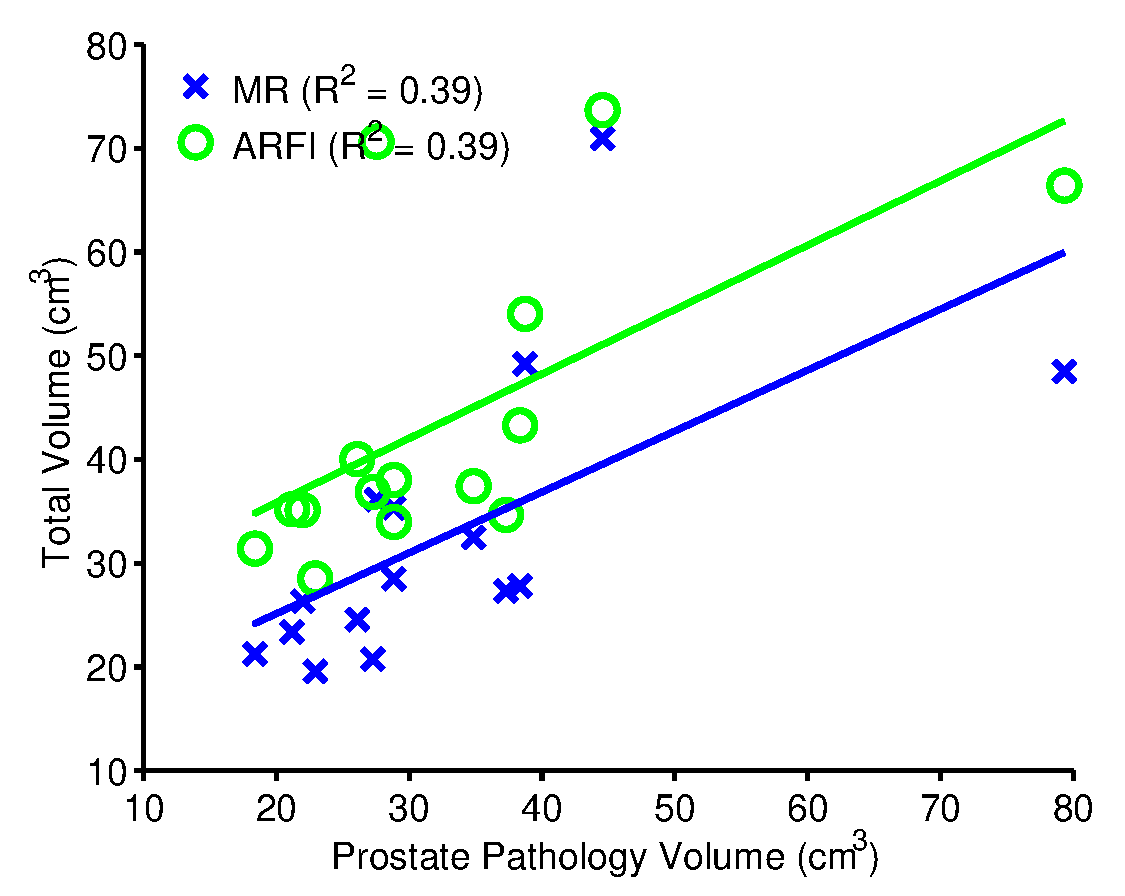
\includegraphics[width=0.3\linewidth]{figs/corr_pathVol_vol_no4} \\
%(d) Image Volume : Prostate Weight (-4) & (e) Image Volume : Path Volume (-4) \\
%\end{tabular}
\caption{Tri-axial pathology measurements were used to make an ellipsoidal
    prostate volume approximation based on gross pathology axis measurements,
    which was moderately well-correlated with the excised prostated weights (a,
    R$^2$ = \pathVolWeightRsq).  T2WI MR (blue, X) showed a moderate
    correlation between the reconstructed volumes and prostate weight (R$^2$ =
    \weightMRrsq), while volumes reconstructed from ARFI images (green, O)
    showed weaker correlation (R$^2$ = \weightARFIrsq) (b).  Weaker
    correlations existed between both T2WI MR and ARFI image volumes and
    approximated ellipsoidal prostate pathology volumes (R$^2$ = \pathVolMRrsq
    and \pathVolARFIrsq, respectively) (c).  One study subject had a very large
    prostate ($>$ 80 g) that was not well visualized by both MR and ARFI
    imaging, and it was excluded from all of the linear regression.  This
    outlier was indicated with magenta circles in the plots.}
\label{fig:mr_arfi_weight}
\end{figure}


\begin{table}
\centering
\caption{Comparison of Central Gland / Zone (C) and Total (T) Prostate Axes in
    MR T2WI and \textbf{B-mode/}ARFI Imaging.  Axes are approximated in orientation to
    match those specified in gross pathology: lateral-to-lateral (LL),
    anterior-to-posterior (AP) and apex-to-base (AB).}
\begin{tabular}{|l|l|l|l|l|l|l|l|l|l|l|l|l|} \hline
{\bf Study} & {\bf MR} & {\bf ARFI} & {\bf MR} & {\bf ARFI} & {\bf MR} & {\bf ARFI} & {\bf MR} & {\bf B-mode} & {\bf MR} & {\bf B-mode} & {\bf MR} & {\bf B-mode} \\ 
{\bf Subject} & {\bf C-AB} & {\bf C-AB} & {\bf C-LL} & {\bf C-LL} & {\bf C-AP} & {\bf C-AP} & {\bf T-AB} & {\bf T-AB} & {\bf T-LL} & {\bf T-LL} & {\bf T-AP} & {\bf T-AP} \\
 & {\bf (cm)} & {\bf (cm)} & {\bf (cm)} & {\bf (cm)} & {\bf (cm)} & {\bf (cm)} & {\bf (cm)} & {\bf (cm)} & {\bf (cm)} & {\bf (cm)} & {\bf (cm)} & {\bf (cm)} \\ \hline
1 & 4.12 & 2.90 & 2.45 & 4.12 & 3.80 & 3.09 & 4.34 & 3.51 & 2.28 & 5.26 & 4.94 & 3.14 \\ 
2 & 3.87 & 3.39 & 2.80 & 3.87 & 4.45 & 3.59 & 4.03 & 3.25 & 1.66 & 3.06 & 5.46 & 3.86 \\ 
3 & 4.82 & 3.48 & 3.27 & 5.11 & 4.11 & 3.59 & 4.53 & 3.23 & 2.29 & 4.53 & 4.55 & 3.68 \\ 
4 & 5.35 & 3.08 & 2.87 & 5.36 & 4.45 & 3.37 & 3.82 & 2.62 & 2.35 & 4.18 & 4.63 & 3.66 \\ 
5 & 6.22 & 4.66 & 4.98 & 7.39 & 5.43 & 5.63 & 5.20 & 5.06 & 2.42 & 5.20 & 6.24 & 4.28 \\ 
6 & 5.05 & 3.44 & 3.44 & 5.10 & 4.84 & 3.44 & 4.63 & 3.96 & 2.29 & 4.50 & 5.83 & 3.10 \\ 
7 & 4.47 & 3.33 & 2.26 & 4.72 & 4.44 & 2.58 & 4.77 & 3.42 & 2.40 & 3.92 & 4.80 & 2.84 \\ 
8 & 4.30 & 3.20 & 2.10 & 4.32 & 4.23 & 2.48 & 5.72 & 4.23 & 2.52 & 4.50 & 4.71 & 2.97 \\ 
9 & 3.52 & 3.31 & 2.19 & 3.52 & 4.33 & 2.70 & 4.73 & 4.90 & 2.69 & 4.43 & 5.71 & 3.06 \\ 
10 & 5.24 & 4.43 & 2.69 & 5.23 & 5.15 & 3.37 & 5.02 & 7.19 & 2.20 & 4.85 & 7.46 & 3.20 \\ 
11 & 5.02 & 3.85 & 2.73 & 5.02 & 5.50 & 3.57 & 4.24 & 4.31 & 2.72 & 3.15 & 5.16 & 2.78 \\ 
12 & 4.55 & 3.70 & 3.30 & 4.58 & 5.38 & 4.24 & 4.24 & 4.63 & 2.34 & 3.87 & 6.74 & 3.83 \\ 
13 & 3.40 & 4.03 & 2.01 & 4.08 & 4.72 & 2.94 & 2.84 & 3.29 & 1.91 & 3.89 & 5.31 & 3.46 \\ 
14 & 3.56 & 3.69 & 2.54 & 3.56 & 4.33 & 3.17 & 4.18 & 4.84 & 2.29 & 4.14 & 5.04 & 3.02 \\ 
15 & 4.79 & 4.17 & 2.56 & 4.95 & 4.69 & 3.32 & 5.00 & 3.78 & 3.08 & 4.12 & 5.31 & 3.60 \\ 
16 & 5.11 & 4.60 & 3.11 & 5.12 & 5.62 & 3.71 & 5.03 & 6.14 & 3.13 & 4.61 & 6.23 & 3.52 \\ 

\hline
\end{tabular}
\label{tab:mr_arfi_axes}
\end{table}

